\subsection{f-HDGM}

\subsubsection{Analysis of relevance of the latent component $\boldsymbol{z}(\boldsymbol{s}, t)$}
 Due to the high computational time which the estimate of the f-HDGM requires, it was not possible to employ the stepwise approach to perform the model selection, therefore starting from the most relevant regressors identified through the estimate of an OLS model, we have built three models with a different number of covariates:
\begin{itemize}
	\item \textbf{large}: \num{9} regressors, i.e. feels-like temperature, rainfall, visibility, wind speed, cloud cover, distance and dummy variables; 
	\item \textbf{medium}: \num{4} covariates, i.e. feels-like temperature, distance and dummy variables;
	\item \textbf{small}: \num{2} regressors, i.e. feels-like temperature and dummy lockdown.
\end{itemize}
 In each of them we have also introduced a constant in order to allow \textbf{D-STEM} to estimate through the EM algorithm the mean number of hourly bike rentals. The aim of this study is to determinate how the relevance of the latent component $\boldsymbol{z}(\boldsymbol{s}, t)$ changes as the number of covariates, i.e. the dimension of $\boldsymbol{\beta}(h)$, varies. In table \ref{V_z_values} are shown the $n_z$ values of the variance of latent component; we can see that variability increases as the model complexity decreases. The reason is the following: if we decide to use a less number of covariates to describe the bike sharing phenomenon, then the descriptive power of $\boldsymbol{z}(\boldsymbol{s}, t)$ increases in order to cope with what the global component $\boldsymbol{x}(\boldsymbol{s}, t, h)' \cdot \boldsymbol{\beta}(h)$ is not able to explain due to reduction of the model complexity.
 
 \begin{table}
 	\centering
 	\renewcommand\arraystretch{1.3}
 	\begin{tabular}{c|c|c|c|c|c|c|c|c}
 		\hline
 		\textit{Model} & \textit{Card.} $\boldsymbol{\beta}(h)$ & $V_{\boldsymbol{z}}^{1,1}$ & $V_{\boldsymbol{z}}^{2,2}$ & $V_{\boldsymbol{z}}^{3,3}$ & $V_{\boldsymbol{z}}^{4,4}$ & $V_{\boldsymbol{z}}^{5,5}$ & $V_{\boldsymbol{z}}^{6,6}$ & $V_{\boldsymbol{z}}^{7,7}$ \\
 		\hline
 		\textbf{Large model} & \num{10} & \num{1.71} & \num{0.75} & \num{1.21} & \num{0.36} & \num{0.65} & \num{0.12} & \num{0.17} \\
 		\hline
 		\textbf{Medium model} & \num{5} & \num{1.93} & \num{0.90} & \num{1.30} & \num{0.38} & \num{0.66} & \num{0.13} & \num{0.19} \\
 		\hline
 		\textbf{Small model} & \num{3} & \num{1.96} & \num{0.93} & \num{1.42} & \num{0.48} & \num{0.79} & \num{0.14} & \num{0.20} \\
 		\hline
 	\end{tabular}
 	\caption[Variances of the latent component $\boldsymbol{z}(\boldsymbol{s}, t)$ as the model complexity varies (f-HDGM)]{variances of the latent component $\boldsymbol{z}(\boldsymbol{s}, t)$, i.e. the main diagonal of the matrix $V_z$, as the model complexity varies, f-HDGM.}
 	\label{V_z_values}
 \end{table}
\noindent
We have decided to describe in detail the \textit{medium model}, a fair compromise between complexity and relevance of the latent component.

\subsubsection{Model parameters}
After having estimated the parameters of the medium model, we have performed the $\chi^2$-test to evaluate the significance of the regressors. Results are shown in table \ref{Chi2_p_values}: all p-values are less than \SI{5}{\percent}, therefore we can conclude all functions $\boldsymbol{\beta}(h)$ related to the chosen covariates are significantly different from zero and consequently give their contribute to explain $\mathit{y}(\boldsymbol{s}, \textit{t}, \textit{h})$, i.e. the number of hourly pickups at a rental station.

\begin{table}
	\centering
	\renewcommand\arraystretch{1.3}
	\begin{tabular}{c|c|c}
		\hline
		\textit{Covariate} & $\chi^2$ \textit{value} & \textit{p-value} \\
		\hline
		\textbf{Constant} & \num{211.16} & $< 10^{-16}$ \\
		\hline
		\textbf{Feels-like temp.} & \num{301.72} & $< 10^{-16}$ \\
		\hline
		\textbf{Distance} & \num{92.83} & $<10^{-16}$ \\
		\hline
		\textbf{Lockdown} & \num{431.19} & $<10^{-16}$ \\
		\hline
		\textbf{Holidays} & \num{32.71} & $4.30 \cdot 10^{-6}$ \\
		\hline
	\end{tabular}
	\caption[p-values of the $\chi^2$-tests to determinate the significance of the regressors (f-HDGM)]{p-values of the $\chi^2$-tests to determinate the significance of the regressors, f-HDGM.}
	\label{Chi2_p_values}
\end{table}

\noindent
In the figure \ref{Trend_beta_M}, instead, we have reported the daily trend of the estimated functions $\boldsymbol{\beta}(h)$ and the variance of $\epsilon$, i.e. $\sigma_{\epsilon}(h)$. It is interesting the trend of $\beta_{const}(h)$ which expresses the mean number of daily pickups during the day; there are two peaks that probably are related with start and end work times. All others variables contribute positively in explaining $y(\boldsymbol{s}, t, h)$, except for the distance and the dummy lockdown; the negative trend of the former is correlated to the fact that an individual is less incentivized to use bike due to tiredness at the end of a working day, that of the latter, instead, is caused to the impossibility to leave own home during the Pause Program in NYC. Moreover, $\beta_{lockdown}$ is also highly uncertain because it's different from zero for only few days. Finally, analysing the behaviour of $\sigma_{\epsilon}(h)$ we can note the estimated model performs worse around 20 o'clock.

\begin{figure}
	\centering
	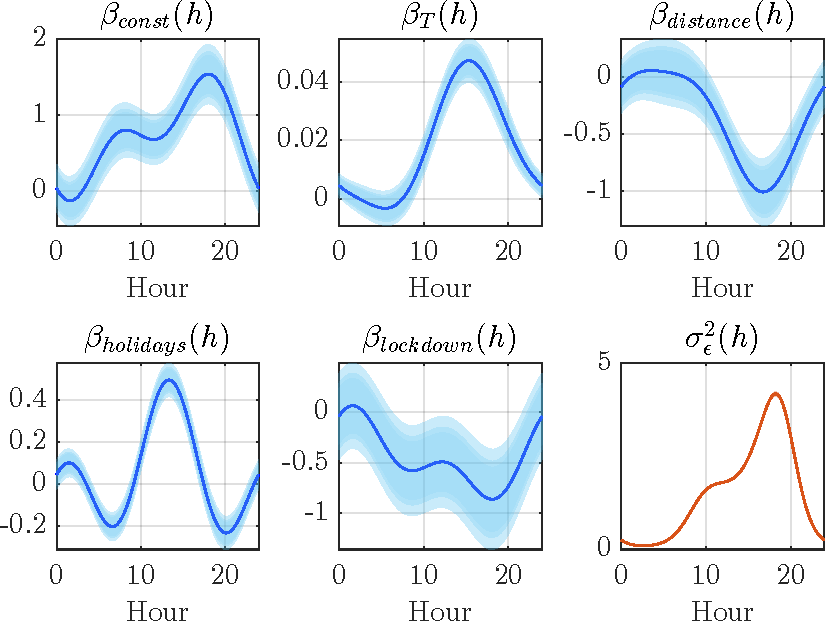
\includegraphics[height=222px]{Images/Data analysis/f-HDGM/Chosen/Trend_beta_M.pdf}
	\caption[Estimated $\beta_{const}(h)$, $\beta_T(h)$, $\beta_{distance}(h)$, $\beta_{holidays}(h)$ and $\beta_{lockdown}(h)$ (f-HDGM)]{estimated $\beta_{const}(h)$, $\beta_T(h)$, $\beta_{distance}(h)$, $\beta_{holidays}(h)$, $\beta_{lockdown}(h)$ and $\sigma_{\epsilon}^2(h)$ with \SI{90}{\percent}, \SI{95}{\percent} and \SI{99}{\percent} confidence bands, respectively, shown through the different shades, f-HDGM.}
	\label{Trend_beta_M}
\end{figure}

\subsubsection{Model validation}
In figure \ref{RMSE_M}, first plot, is shown the trend of RMSE$_h$ and RMS$_h$; thanks to the latter differences are accentuated, therefore we can note as the medium model in validation performs worse in peak hours. Dotted line describes the case in which we round $\hat{y}(\boldsymbol{s}, t, h)$ to the nearest integer. In the second plot, instead, is shown the behaviour of RMSE$_t$ during \num{2020}; we can notice the period in which the estimated model performs worse is in summer, however the range of values assumed by this statistical index is not wide, therefore differences between means in each period are not particularly marked. Finally, in figure \ref{RMSE_comp} is reported a comparison between the behaviours in validation of the three estimated models; albeit slightly we can note that the small model is the best because probably, thanks to his reduced complexity, doesn't go into overfitting. We please you to read table \ref{RMSE_f-HDGM_stats} for more information concerning RMSE$_h$, RMSE$_t$ and RMSE$_s$.

\begin{figure}
	\centering
	\subfigure[]{\label{RMSE_M}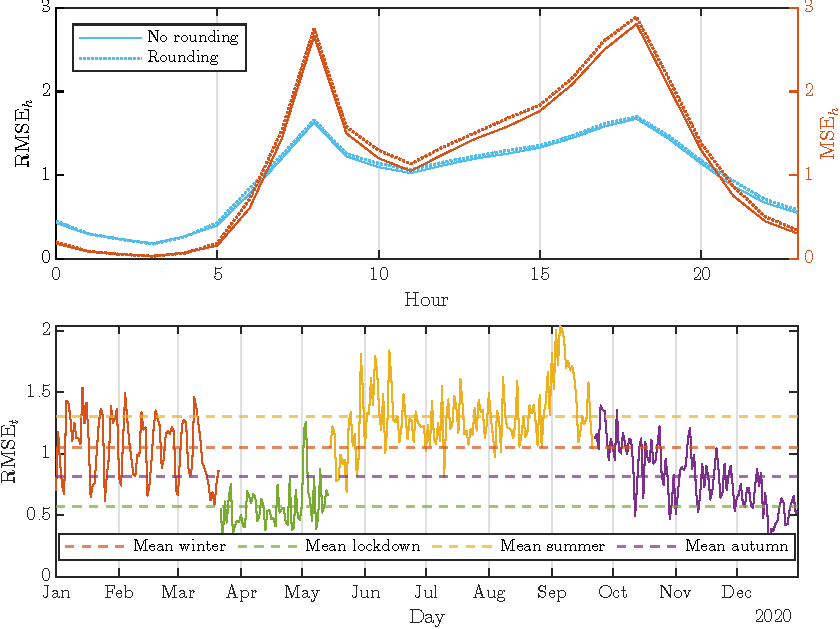
\includegraphics[height=177px]{Images/Data analysis/f-HDGM/Chosen/RMSE_M}}\quad
	\subfigure[]{\label{RMSE_comp}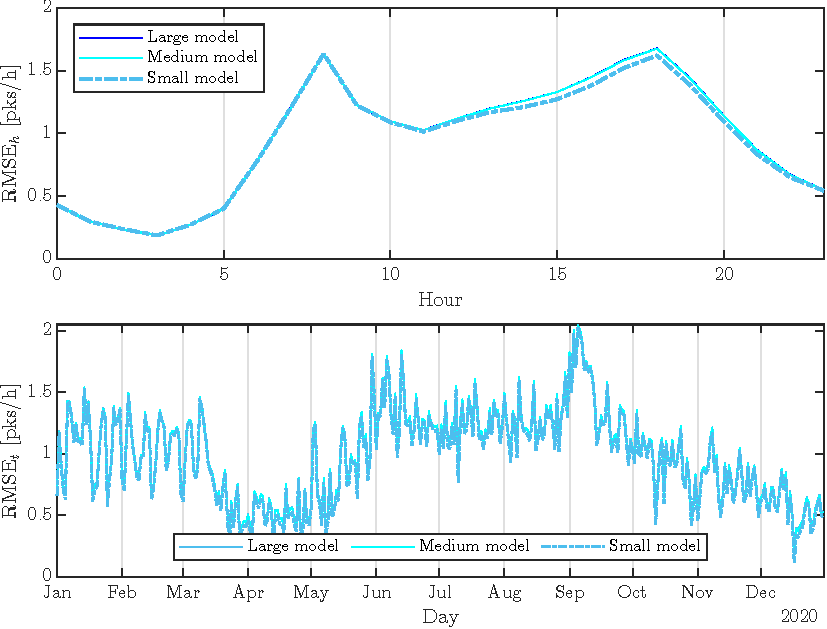
\includegraphics[height=177px]{Images/Data analysis/f-HDGM/Chosen/RMSE_comp}}\quad
	\caption[Trends of RMSE$_h$ and RMSE$_t$ concerning medium model and comparison between the behaviours in validation of the three estimated models (f-HDGM)]{trends of RMSE$_h$ and RMSE$_t$ concerning medium model (a) and comparison between the behaviours in validation of the three estimated models, f-HDGM.}
\end{figure}

\begin{table}
	\centering
	\renewcommand\arraystretch{1.3}
	\begin{tabular}{c|c|c|c|c|c}
		\hline
		\textit{Index} & \textit{Min.} & \textit{Max.} & \textit{Mean} & \textit{Median} & \textit{Std}\\
		\hline
		\textbf{Hourly RMSE$_h$} & \num{0.19} & \num{1.68} & \num{0.96} & \num{1.11} & \num{0.48}\\
		\hline
		\textbf{Hourly RMSE$_t$} & \num{0.22} & \num{2.04} & \num{1} & \num{1.04} & \num{0.36} \\
		\hline
		\textbf{Hourly RMSE$_s$} & \num{0.44} & \num{2.17} & \num{1} & \num{0.96} & \num{0.40}\\
		\hline
	\end{tabular}
	\caption[Main statistics concerning RMSE (f-HDGM)]{main statistics concerning RMSE, f-HDGM.}
	\label{RMSE_f-HDGM_stats}
\end{table}